\section{Methodology}
\label{sec:method}

%We now present the proposed TER model, which uses temporary information for 
%explanation recommendation.

%============================================================================
%
%We now describe the proposed \tkgrec\ in details.
% Figure \ref{pipeline} sketches the model's architecture, which 
%consists of four main modules: 
%%
%\textbf{(1) Time-aware interact} 
%module, which constructs TKG by the interaction time-series 
%clustering mechanism and encodes the TKG to get temporal representation;
%%
%\textbf{(2) Time-aware Path Reasoner} 
%module, which innovatively leverages temporal information as guiding signals 
%for generating personalized recommendation; 
%%
%\textbf{(3) Temporal Ranking Recommendation} 
%module, which aims at ranking the predicted items from the trained reasoner to 
%get a temporal order recommendation.
In this section, we introduce the proposed \tkgrec\ in detail.
The overall framework of time-aware path reasoning is shown in Figure 
\ref{pipeline}.
%
Our approach is able to effectively fuse temporal information into knowledge 
graph and leverage a RL framework for recommendation.
In what follows, we start with 
\textbf{Time-aware Interaction Relation Extraction} 
to construct TCKG, and use \textbf{Time-aware representation learning} 
to generate entities and relations representations.
Then we present \textbf{Time-aware Path Reasoning} and \textbf{Model Prediction} to reason over TCKG for recommendation.

%============================================================================



\subsection{Time-aware Interaction Relation Extraction}\label{tire}
Clearly, how to deal with the dynamic characteristics of user-item interactions is of crucial importance in our task.
However, simply treating the interaction timestamps as auxiliary features might limit the potential of time-aware reasoning, due to the following challenges:
(1) As the timestamps are usually numerous \cite{datasetAmazon}, directly attaching them with user behaviors might cause meaningless features, such as purchase\_20150101 and purchase\_20150102, thus enlarging the feature space dramatically and losing the periodic semantics of timestamps.
(2) The interaction graph and knowledge graph come from heterogeneous sources, and thus are hardly updated synchronously --- that is, the interactions are usually dynamic, while the item knowledge (\eg, category, brand) is fixed over different timestamps.

To solve these challenges, we first consider the temporal and behavioral characteristics of interactions by projecting the timestamps into a temporal feature space $\mathcal{T}$.
It encodes temporal statistical and temporal structural features of interaction timestamps.
We then group the interaction timestamps $T = \{t_1, t_2, \cdots, t_n\}$ into $L$ categories, and then extend the single interaction type into $\mathcal{V}_{\mathcal{U}}^T = \{ \mathcal{V}_{\mathcal{U}}^1, \mathcal{V}_{\mathcal{U}}^2, \cdots, \mathcal{V}_{\mathcal{U}}^{L} \}$.
After that, the temporal user-item graph can be seamlessly integrated with relatively static KG based on the item-entity alignment set, and finally get the TCKG we need.
The extraction process is illustrated in Figure \ref{clu}.


% we first group the interaction timestamps $T = \{t_1, t_2, \cdots, t_n\}$ into $l$ categories, and then extend the single interaction type into $\mathcal{V}_{\mathcal{U}}^T = \{ \mathcal{V}_{\mathcal{U}}^1, \mathcal{V}_{\mathcal{U}}^2, \cdots, \mathcal{V}_{\mathcal{U}}^{l} \}$.
% Thereafter, we consider the temporal and behavioral characteristics of interactions by projecting the timestamps into a feature space $\mathcal{T} \in \mathbb{R}^m$, where $m$ indicates the space dimension.
% It encodes temporal statistical and temporal structural features of interaction timestamps.
% We illustrate the extraction process in Figure \ref{clu} and and elaborate it in the next sections. 



% Directly treating the timestamp as auxiliary features of the entity or 
% relation is suboptimal for path reasoning, due to the 
% following challenges:
% (1) As the timestamps are usually numerous \cite{datasetAmazon}, simply attaching the original relation with timestamps might loss the periodic characteristics and lead to meaningless features.
% (2) More importantly, the user-item bipartite graph and knowledge 
% graph come from different sources and are hardly updated synchronously --- that is, the interactions are dynamic, while the item knowledge (\eg, category, brand) is static over different timestamps.
% % The interaction of users purchasing items is happening all the time, and every interaction occurs with explicit behavioral intentions. But the external knowledge graph is derived from existing public KGs or extracted from 
% % the local business information network (\eg, category, brand), which is 
% % difficult to capture complete and specific timestamps.
% %
% Here, we propose TCKG to emphasize the dynamics of interactions.
% In particular, we divide the timestamps of interactions $T = \{t_1, 
% t_2, \cdots, t_n\}$ into $l$ categories, and obtain the time-aware interaction relations $\mathcal{V}_{\mathcal{U}}^T = \{ \mathcal{V}_{\mathcal{U}}^1, \mathcal{V}_{\mathcal{U}}^2, \cdots, \mathcal{V}_{\mathcal{U}}^{l} \}$.
% We visualize the extraction process in Figure \ref{clu}.
 
% To capture the temporal and behavioral characteristics of interactions, we identify two types of discriminative features: \textit{statistical} features and 
% \textit{structural} features.
% %
% These two types of features 
% %are widely used in unlabeled time-series data \cite{features_time},
% will represent 
% interaction timestamp set $T = \{t_1, t_2, ..., t_n\}$
% and compose our temporal feature space  $\mathcal{T} \in \mathbb{R}^m$, 
% where $m$ indicates the 
% dimensionality of the space.
% The details will be shown below.



\subsubsection{\textbf{Temporal Statistical Features}}
Before clustering timestamps, we project them into a feature space.
Specifically, the statistical features are considered to capture some time rules like seasonal changes, periodic purchases \cite{liao2005clustering}.
Hence, for a specific timestamp $t$, its statistical feature is formally summarized as:
\begin{equation}
    \boldsymbol{f}_{stat} =year(t)|| season(t) || month(t) || week(t) \cdots,
\end{equation}
where $\boldsymbol{f}_{stat}$ encodes the year,  season, month, week, and other statistical characteristics of $t$ and concatenates them together, where $||$ is the concatenate operator.


\begin{figure}[tb]
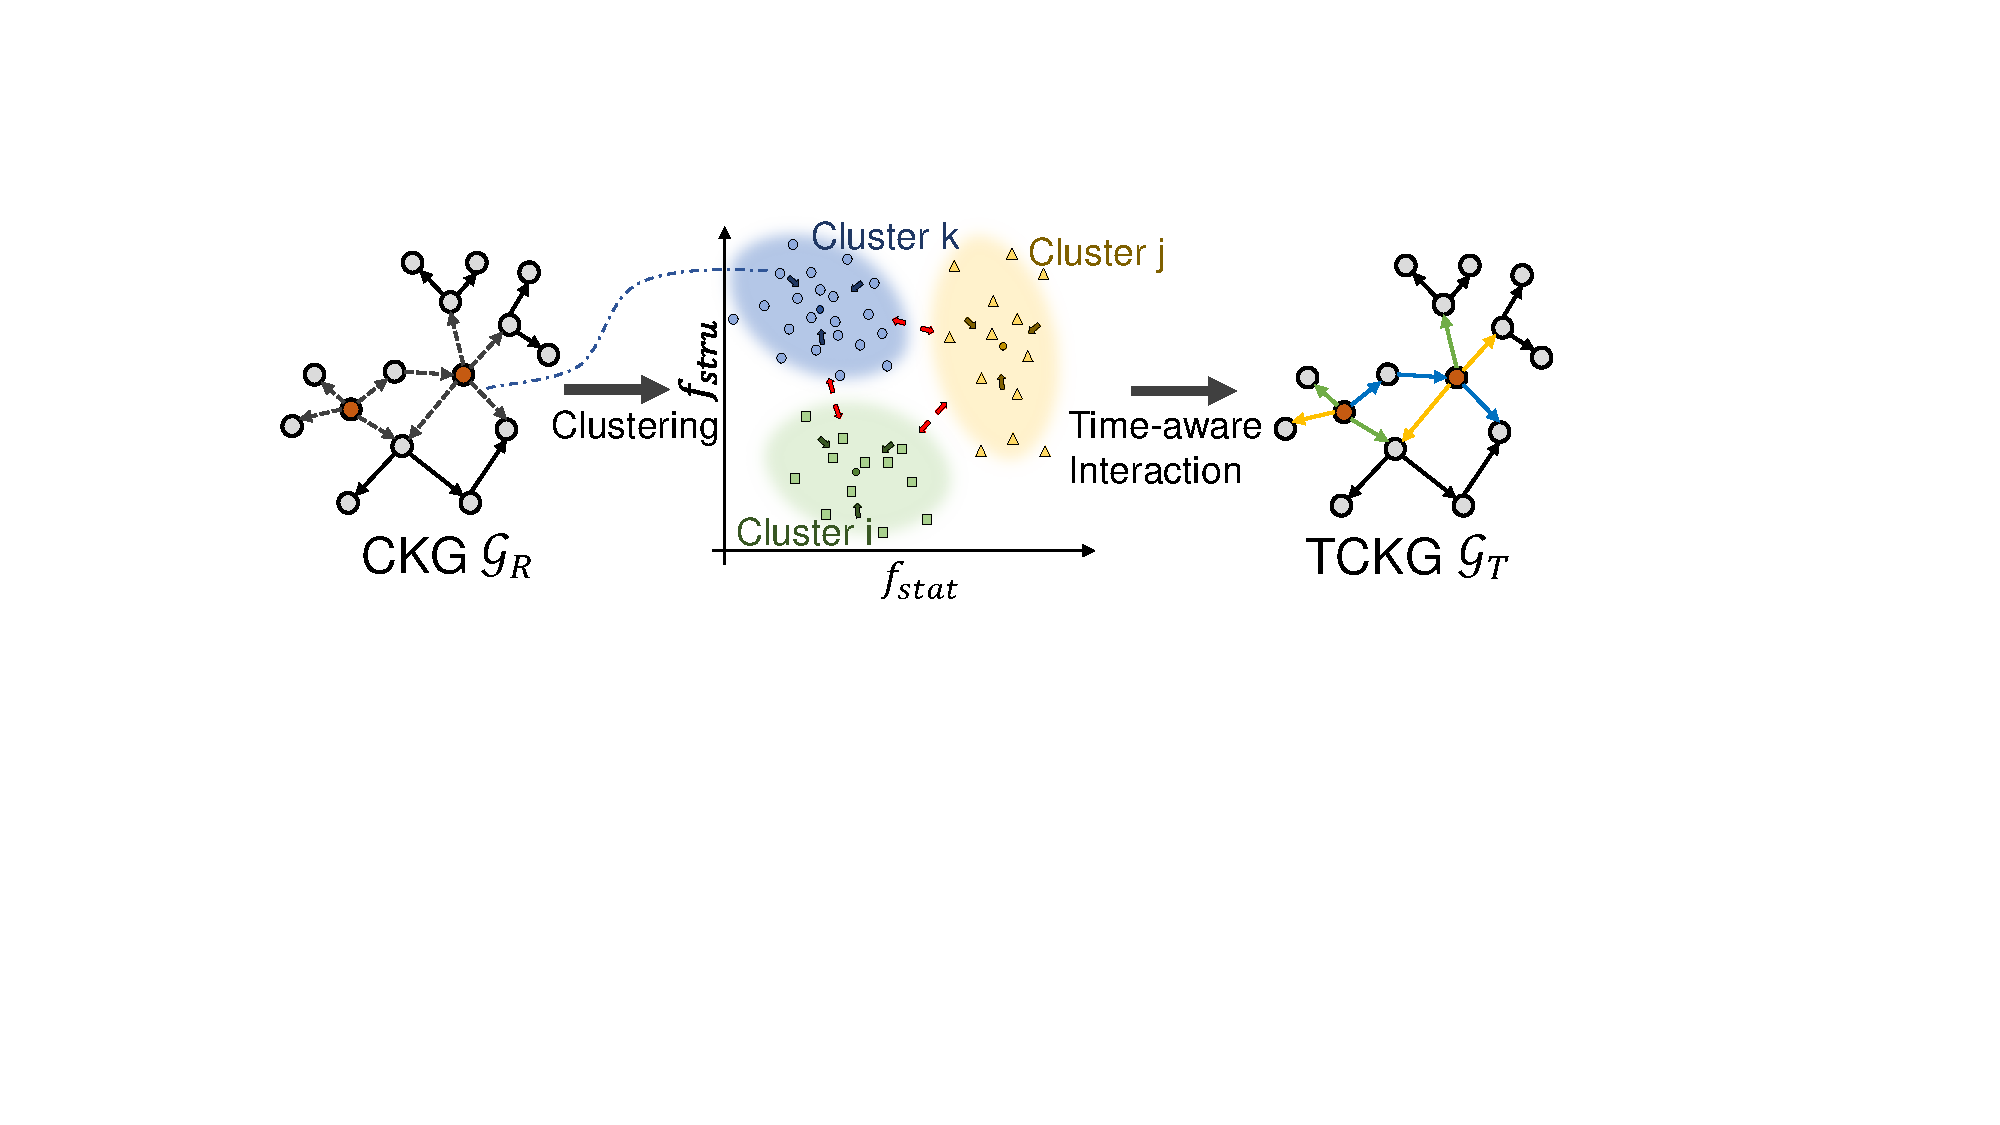
\includegraphics[width=0.85\columnwidth]{chart/clu.pdf}
\caption{Process of time-aware interaction relation extraction. Each 
interaction relation's (dashed edge) timestamp will be mapped into temporal 
feature space 
$\mathcal{T}$ and clustered. Different colored edges (\eg, blue, yellow, green) in TCKG represent 
different clustering results. }
\label{clu}
\end{figure}

\subsubsection{\textbf{Temporal structural features}}
Beyond the statistical features, we also exploit the structural features to delineate the characteristics of user behaviors, which measures the purchase propensity (\eg, shopping festival) at timestamp $t$.
More formally, we define the structural feature of $t$ as:
\begin{equation}
	\boldsymbol{f}_{stru} = z_{gap}'(t) || z_{gap}''(t),
\end{equation}
where $z_{gap}'(t)$ is the first-order structural feature, which measures the trend of interaction number in the current $gap$ time, compared with that in the past $gap$; $gap$ represents the granularity of window period, which can be set as 30 (\ie, month), or 1 (\ie, day); analogously, $z_{gap}''(t)$ denotes the second-order structural feature and models the momentum of interaction trend.
More formally, $z_{gap}'(t)$ and $z_{gap}''(t)$ is defined as:
% \begin{equation}
% 	 z_{gap}'(t) = \frac{\sum_{i=t-gap}^{t}z(i) - \sum_{i=t-2gap}^{t-gap}z(i)}{gap}
% \end{equation}
\begin{align}  \label{z_p}
	 z_{gap}'(t) &= \frac{\sum_{i=t-gap}^{t}z(i) - \sum_{i=t-2gap}^{t-gap}z(i)}{gap},\ & z_{gap}''(t) &= \frac{\sum_{i=t-gap}^{t}z_{gap}'(i) - \sum_{i=t-2gap}^{t-gap}z_{gap}'(i)}{gap},
\end{align}

where $z(i)$ is the interaction number happened on timestamp $i$, and we replace $z(i)$ with $z_{gap}'(i)$ in Eq. \ref{z_p} to calculate $z_{gap}''(t)$.
For those timestamp $t$ has less than $2gap$ historical interactions, their historical information is not enough to calculate $z_{gap}'(i)$.
In that case, we padding their corresponding features with the nearest timestamp's temporal structural feature. The same goes for $z_{gap}''(t)$.
% We replace it with the nearest timestamp
% As a result, $\boldsymbol{F}^{\prime \prime}$ reflects the first-
In this work, we set the gap as 90 (\ie, season), 30 (\ie, month), 7 (\ie, week), 1 (\ie, day) and simply concatenate them as temporal structural features.

Thereafter, we combine these two features together as the temporal feature space $\mathcal{T} \in \Space{R}^m$ for timestamp $t$:
\begin{equation}
	\mathcal{T} = \boldsymbol{f}_{stat} \ || \ \boldsymbol{f}_{stru},
\end{equation}
where $m$ is the feature dimension.


% Before grouping timestamps into categories, we map them into temporal feature 
% space 
% $\mathcal{T}$. The statistical features are 
% expected \cite{liao2005clustering} to capture some time rules like seasonal 
% changes, periodic 
% purchases, 
% \etc\ 
% The statistical features can be formally summarized as:
% \begin{equation}
% 	\boldsymbol{F}^{\prime} = f_{stat}(t)
% 	\end{equation}
% 	where $t$ represent an interaction timestamp, and $f_{stat}(t)$ means 
% 	encode 	the 
% 	timestamp $t$ with statistical features. 
% 	\ie, the function $f_{stat}(\cdot)$ will extract 
%  the year, month, season, week and other statistical characteristics of 
% each timestamp $t$, and concatenate them together after encoding. In particular, 
% $f_{stat}$
% can be formulated as:
% \begin{equation}
% 	f_{stat}(t) = year(t) \| season(t) \| month(t) \| ... 
% 	\end{equation}
% 	where $\|$ means concatenate operator.



% \subsubsection{Temporal structural features}
% Beyond the statistical features, we exploit structural features to capture 
% the characteristics of users' shopping behavior.
% Similarly, the statistical features can be formulated as:
% \begin{equation}
% 	\boldsymbol{F}^{\prime \prime} = f_{stru}(t)
% 	\end{equation}
% More specifically, $f_{stru}(t)$ contains 
% the first- and second-order features
% of time-interact function $z(t)$:
% \begin{equation}
% 	f_{stru}(t) = z_{gap}^{\prime}(t)  \| 
% 	z_{gap}^{\prime \prime}(t)
% 	\end{equation}
% where time-interact function $z(t)$ is the interaction number $n$ occured on 
% timestamp $t$, and $z_{gap}^{\prime}(n)$ model the trend of $n$ in current 
% $gap$ 
% time relative to past $gap$ time:
% \begin{equation}
% 	 z_{gap}^{\prime}(t) = \frac{\sum_{i=t-gap}^{t}z(i) 
% 	 - \sum_{i=t-2gap}^{t-gap}z(i)}{gap}
% 	\end{equation}\label{z_p}
% where $gap$ represents time granularity, which can be 30 (\ie month), 90 (\ie 
% season) or 1 (\ie day), \etc\ $z_{gap}^{\prime \prime}(t)$ models the momentum 
% of interaction trend, and can be calculated by replacing $z(i)$ in Equation 
% \ref{z_p} with $z_{gap}^{\prime}(t)$.

% These two types of features will compose our time-aware feature space 
% $\mathcal{T} \in 
% \mathbb{R}^m$:
% \begin{equation}
% 	\mathcal{T} = \boldsymbol{F}^{\prime} \|  \boldsymbol{F}^{\prime \prime}
% 	\end{equation}

\subsubsection{\textbf{TCKG Construction}}
Having mapped the timestamp to the temporal feature space, we now construct the relation of time-aware interaction.
Here we adopt a time-series clustering method, Gaussian Mixture Model (GMM) \cite{gmm}, on the timestamp set $T$, so as to reduce the timestamp numbers and discretize them into group values.
We leave the exploration of other clustering methods, such as K-means \cite{kmeans}, DBSCAN \cite{ester1996density}, and Mean-shift \cite{meanshift}, in future work.

Specifically, we hire $L$ Gaussian models. For the timestamp $t$ with its temporal feature, we can get the probability $w_{l}$ of being generated by the $l$-th Gaussian model.
As such, the interaction relation $r_t$ on timestamp $t$ can be obtained as follows:
\begin{equation}\label{relation_cluster_2}
	r_t \leftarrow \Space{I}_{max(\Mat{W}_{t})}(\Mat{W}_{t}) {\mathcal{V}_{\mathcal{U}}^T} \ ,
\end{equation}
where $\Mat{W}_{t} = [w^{1}_t, w^{2}_t, \cdots, w^{L}_t]^{\mathsf{T}}$ indicates the $t$-specific probability distribution derived from the Gaussian models;
${\mathcal{V}}_{\mathcal{U}}^T = [\mathcal{V}_{\mathcal{U}}^1, \mathcal{V}_{\mathcal{U}}^2, \cdots, \mathcal{V}_{\mathcal{U}}^{L}]$ is the time-aware interaction relation set, where $\mathcal{V}_{\mathcal{U}}^{l}$ is the $l$-th clustered relation.
Equation \eqref{relation_cluster_2} replaces $r_t$ with the most probable relation in ${\mathcal{V}}_{\mathcal{U}}^T$.
The number of time clusters $L$ is determined by the Bayesian Information Criterion (BIC) \cite{bic}, which is adjusted adaptively for different datasets.


Through the above extract process, we are able to project each observed interaction with timestamp into the same time-aware feature space, and divide all timestamps into weighted $L$ clusters by GMM.
The clustering assignments are used to replace the original interaction relations in CKG and finally convert CKG into TCKG.


% \subsubsection{TCKG Construction}
% Having mapped  the timestamp set $T$ to the time-aware feature space 
% $\mathcal{T}$, 
% we need to construct a time-aware interact relation based on those information.
% Here we adopt a time-series clustering mechanism on timestamp set $T$
% because the total number
% of timestamps is numerous and need to be bucketized into group values.
% % 表示很多聚类方法也行但是我们用的是GMM做.
% The clustering process can be modeled by K-means \cite{kmeans}, DBSCAN 
% \cite{ester1996density}, or 
% Mean-shift \cite{meanshift}, \etc\
% Intuitively, we integrate a simple but effective Gaussian Mixture 
% Model (GMM) \cite{gmm} to cluster time data. 



% Especially, for each $i$-th time vector 
% $\boldsymbol{t}_i \in \mathbb{R}^m$, we can get the probability $w_i(k)$ of 
% being generated by the $k$-th Gaussian model (the total amount is $l$). The 
% interaction relation 
% $\boldsymbol{r}_{t_i}$ on $t_i$  can be expressed as follows:
% \begin{equation}
% 	\boldsymbol{r}_{t_i} \leftarrow 
% 	\mathbb{I}_{max(\boldsymbol{w}_i)}(\boldsymbol{w}_i)
% 	\boldsymbol{R}_L^\intercal, \label{relation_cluster_2}
% 	\end{equation}
% where $\boldsymbol{w}_i = [w_i(1), w_i(2), ..., 
% w_i(l)]$ indicates the probability of $\boldsymbol{t}_i$ for each
% Gaussian model, and $\boldsymbol{R}_L = [r_{1}, 
% r_{2}, ..., r_{l}]$ is the extended relation set clustered 
% by GMM where $r_{l}$ is the $l$-th clustered relation. 
% Equation (\ref{relation_cluster_2}) means replacing $\boldsymbol{r}_{t_i}$ with 
% the most 
% probable relation in $\boldsymbol{R}_L$. 
% The number of time clusters $l$ is determined 
% by the Bayesian Information Criterion
% (BIC) \cite{bic},  
% which is adjusted adaptively for different datasets. 
	

% Therefore, each observed interaction with timestamp could be projected into  
% time-aware feature space 
% $\mathcal{T}$, and then be divided into weighted $l$ clusters by GMM model. 
% Those clustered result will replace the original interaction relations in CKG 
% and finally contributes to constructing TCKG.

\begin{figure}[tb]
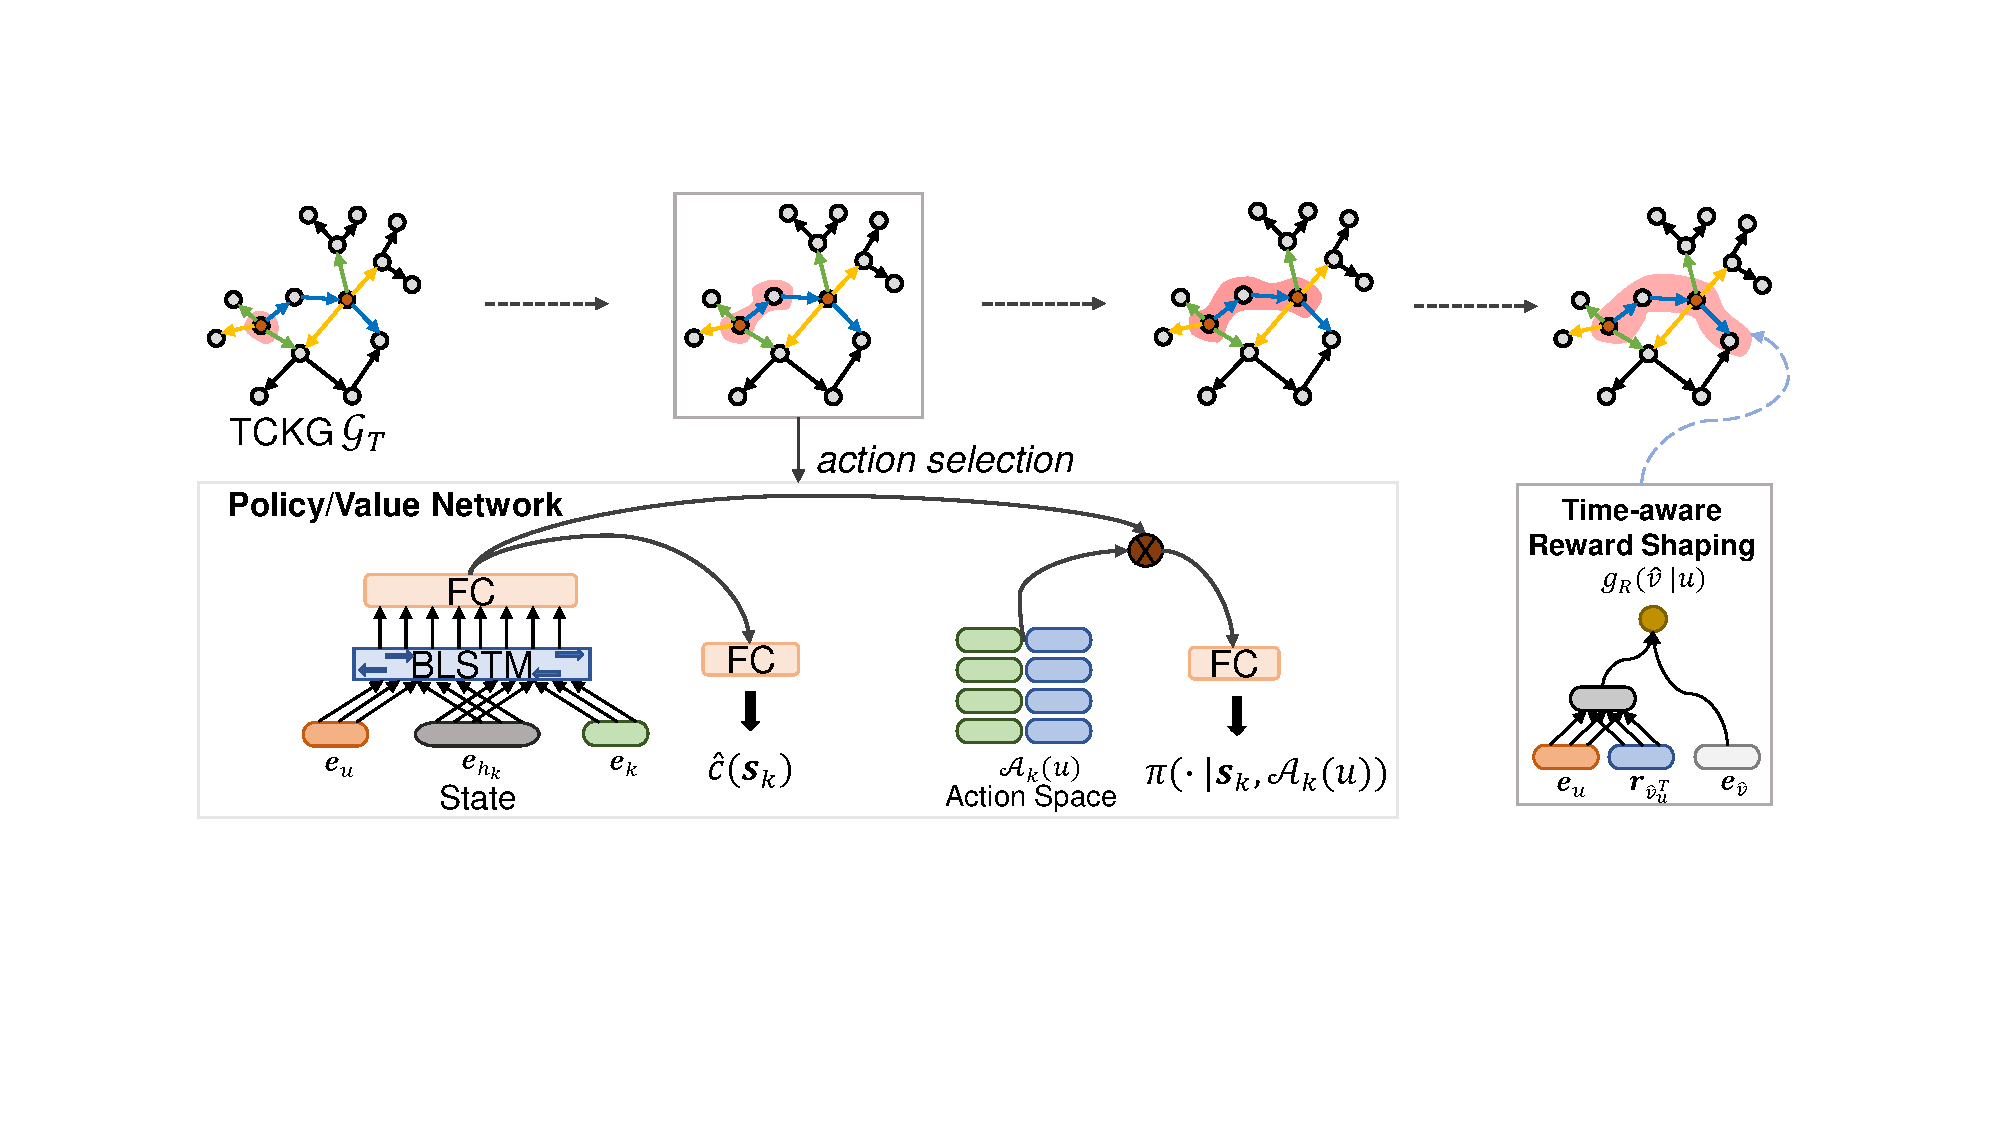
\includegraphics[width=\columnwidth]{chart/pipelineMH.pdf}
\caption{ Overall training approach of the proposed \tkgrec\ model.
		For a user $u$ at each time step $k$, as shown in the pink shaded part of TCKG, the agent chooses the next hop based on the temporal constraint, which samples a  
		link $a_k$ according to 
		$\pi\left(\cdot \mid \mathbf{s}_k, \mathcal{A}_{k}(u)\right)$.
		The agent receives a reward $g_R(\hat{v} \mid u)$  when stopped at an item 
		$\hat{v}$. The pink shaded path starts at user $u$ and ends at item $\hat{v}$, showing why our \tkgrec\ model recommends $\hat{v}$ to $u$.
		%
%		Framework overview of the proposed \tkgrec\ model. 
%				The algorithm aims to learn a policy that navigates from
				}
		\label{pipeline}
\end{figure}



\subsection{Time-aware Representation Learning}\label{trl}
Having constructed TCKG, we aim to learn representations for entities and relations by exhibiting the structural and temporal information.
In particular, the KG relations (defined as $r_{kg}$) require the entity representations to meet the structural constraints and maintain the semantics, while the time-aware interaction relations (defined as $r_{interact} \in {\mathcal{V}}_{\mathcal{U}}^T $) encourage the relation affinity within the same categories compared to that of different categories.



Towards this end, we employ the widely-used knowledge graph embedding method, TransE \cite{transE}, on TCKG.
To be more specific, for a given TCKG triplet $(h,r,t)$, it represents head entity $h$, relation $r \in \{r_{kg} \cup r_{interact}\}$ 
% which includes external KG relation $r_{kg}$ and interact relation $r_{interact}$
, and tail entity $t$ with $d$-dimension embeddings, \ie, $\Mat{e}_{h}$, $\Mat{r}$, $\Mat{e}_{t}$ $\in \mathbb{R}^d$.
These embeddings follow the translational principle: $\Mat{e}_h + \Mat{r} \approx \Mat{e}_t$.
Hence,  for a given triplet $(h, r, t)$, the scoring function is defined as the distance between $\Mat{e}_h + \Mat{r}$ and $\Mat{e}_t$, \ie,
\begin{equation}\label{trans}
	g_{r}({h},{t})=\|\Mat{e}_h+\Mat{r}-
	\Mat{e}_t\|_2^2 .
\end{equation}
A smaller score $g_{r}(h, t)$ suggests that the fact $(h, r, t)$ is more likely to be true, and vice versa. 
We employ the pairwise loss function to train the TCKG embeddings, which accounts for the relative order between the valid triplets and broken ones:
\begin{equation}\label{eqtranse}
    \Lapl_{tckg}=\sum_{\left(h, r, t, t'\right) \in \Set{S}}-\ln\sigma\left(g_{r}({h},{t}') - g_{r}({h},{t})\right)
\end{equation}
where $\Set{S} = \{(h, r, t, t') | (h, r, t) \in \Set{G}_T, (h, r, t') \notin \Set{G}_T\}$, and $ (h, r, t')$ is collected with the tail $t$ replaced by a random entity $t'$; 
$\sigma(\cdot)$ is the sigmoid function. 
This loss serves as a constraint that injects the structural and temporal information into representations, thus preserving the semantics of entities and relations.



% Having constructed the TCKG, we learn 
% representations for entities and relations by jointly considering inherent 
% graph structure and temporal information.
% %
% Therefore, our learning procedure of TCKG embedding comes from \textbf{two} 
% signals: (i) 
% \textbf{Original KG relations}, which makes embedding meet the
% semantic and structural constraints; and (ii) \textbf{Time-aware interaction 
% relations}, 
% which reduces the distances between time-aware relations
% $\mathcal{V}_{\mathcal{U}}^T$ of the same categories and increases the distances
% between the relations of different categories. 


% According to former Section \ref{tire}, our TCKG's relation types 
% $\mathcal{R}_T$ are 
% composed of two categories: original KG relations $r_{kg} \in 
%  \mathcal{R}$ and time-aware interaction relations  $r_{interact} \in \{ 
%  \mathcal{V}_{\mathcal{U}}^1, 
%   \mathcal{V}_{\mathcal{U}}^2, 
%   ..., \mathcal{V}_{\mathcal{U}}^{l} \}$. Although they are both relation types 
%   in TCKG, those embedding distances between $\boldsymbol{r}_{kg}$ and 
%   $\boldsymbol{r}_{interact}$ need to be different. 
% %
% For example, assuming that there are relations $\{r_{a1}, r_{a2}, r_{b1}, 
% r_{b2}\}$ extracted from relations $A$ and $B$. 
% In addition to be encoded by translational distance, furthermore, the distance 
% of
% relation embeddings extracted from the same relation type should be smaller 
% than those from different relation types, \eg, $ \text{d}(\boldsymbol{r}_{a1}, 
% \boldsymbol{r}_{a2}) \leq 
% \min(\text{d}(\boldsymbol{r}_{ai}, \boldsymbol{r}_{bj}))$, $\text{where} \  
% i,j=1,2$, and $\text{d}(\cdot)$ measures distance. 

% We employ the translational scoring function 
% \cite{transE}, 
% a widely used embedding method, on TCKG. To be more specific, it represents 
% both entities and relations in $d$-dimension 
% vector space, \ie, $\boldsymbol{e}_h, \boldsymbol{e}_t, \boldsymbol{r} \in 
% \mathbb{R}^d$, and 
%  makes embeddings follow the translational principle: $\boldsymbol{e}_h + 
%  \boldsymbol{r} \approx \boldsymbol{e}_t$, where $\boldsymbol{e}_h, 
%  \boldsymbol{e}_t$ are the head and tail entity embeddings, and 
%  $\boldsymbol{r} \in \{ 
%  \boldsymbol{r}_{kg} \cup \boldsymbol{r}_{interact}  \}$ 
%  is the relation embedding.
%  %
%  Hence,  for a 
%  given triplet $(h, r, t)$, the scoring 
%  function is defined as the 
%  distance between $\boldsymbol{e}_h + 
%   \boldsymbol{r}$ and $\boldsymbol{e}_t$, \ie,
% 	 \begin{equation}
% 	g_{r}({h},{t})=\|\boldsymbol{e}_h+\boldsymbol{r}-
% 	\boldsymbol{e}_t\|_2^2 ,
% 		 \end{equation} \label{trans}
%  A larger score $g_{r}(h, t)$ suggests that the fact $(h, r, t)$ is more likely 
%  to 
%  be true, and vice versa. 
 %
 %
%  In this way, the original KG relations $r_{kg}$ will be directly encoded by 
%  translational constraint.
% % as 
% % translational representation, because their positions in TCKG are still in 
% % their original places.
%  %
%  As to time-aware interaction relations $r_{interact}$, those relations 
%  extracted  from the 
%  same  interaction relation connect with same head entity types and tail entity 
%  types.  Therefore, the distance of their  
%  representation are smaller than those extracted from different interaction 
%  relation.
%  % 
%  %
%  The training of TCKG embedding considers the relative 
%  order between valid triplets and broken ones, and encourages
%  their discrimination through a pairwise ranking loss:

% \begin{equation}\label{eqtranse}
% \mathcal{L}_{tckg}=\sum_{\left(h, r, t, t^{\prime}\right) \in \mathcal{S}}-\ln 
% \sigma\left(g_{r}({h},{t}^{\prime}) - g_{r}({h},{t})\right)
% \end{equation}
% where $S = \{(h, r, t, t^{\prime}) | (h, r, t) \in \mathcal{G}_T, (h, r, 
% t^{\prime}) \notin \mathcal{G}_T\}$, and $ (h, r, t^{\prime})$ is collected 
%  with the tail $t$ replaced by a random entity $t^{\prime}$.
% $\sigma(\cdot)$ is the sigmoid function. 
% % original KG relations 因为仍然保留了原有的状态, 因此嵌入学习不变.
% % time-aware interaction relations, 由相同interaction提取出的relation之间,头尾实体
% %类别相似, 因此尽管它们在TCKG中属于不同的relation type, 
% %它们的distance会比不同interaction提取的relation更远. 因此完成我们的time-aware 
% %representaion.
% This loss serves as a 
% constraint signal, injecting the direct connections and temporal information 
% into representations, and 
% thus increases the semantics in the embedding .




%
%\subsubsection{Metric Learning.} 
%According to former Section \ref{tire}, our TKG's relation types are 
%composed of two categories: original KG relations $\mathcal{R}$ and temporal 
%classified relations $\mathcal{R}_T$. Although they are both relation types in 
%TKG, those 
%embedding distances between them need to be different. 
%%
%For example, assuming that there are relations $\{a_1, a_2, b_1, b_2\}$ 
%extracted from 
%relations $A$ and $B$. 
%In addition to be encoded by translational distance, furthermore, the distance 
%of
%relation embeddings extracted from the same relation type should be smaller 
%than those from different relation types, \eg, $ \text{d}(a_1, a_2) \leq 
%\min(\text{d}(a_i, b_j))$, $\text{where} \  i,j=1,2$, and $\text{d}(\cdot)$ 
%measures 
%distance. 
%
%In this way, those entities and relations can still encode their original 
%type  
%information into their embedding after being clustered by time, which couples 
%temporal information with types connection to achieve richer 
%representation.
%
%
%
%In order to make Euclidean distances between feature vectors from different 
%classes larger than that from the same class, inspired by 
%\cite{triloss},  
%we set TriHard loss to constraint:
%	\begin{equation}\label{eqtri}
%	\mathcal{L}_{T H}=\sum_{sa\in D, p_{h}, 
%	n_{h}}\left[\text{d}\left(\boldsymbol{r}_{sa}, 
%	\boldsymbol{r}_{p_h}\right)-\text{d}\left(\boldsymbol{r}_{sa}, 
%	\boldsymbol{r}_{n_h}\right)+\alpha\right]_{+}(\alpha>0)
%	\end{equation}
%where $\text{d}(x,y)$ represents the Euclidean distance between $x$ and $y$, 
%$\boldsymbol{r}_{sa} 
%\in \mathbb{R}^d$ are relation embedding vectors of 
%samples in mini-batch $D$, $\boldsymbol{r}_{p_h}, \boldsymbol{r}_{n_h} \in 
%\mathbb{R}^d$ are relation embedding vectors of the hardest positive and 
%negative samples towards anchors within $D$, and $\alpha$ is the margin. It 
%makes 
%the hardest relation triplets 
%more soft and various, and simultaneously solves the distance problem by 
%making 
%the anchor converge to 
%local minima.
%
%In addition to keeping the embeddings of different classes separable, 
%\cite{centloss} is utilized
%here for minimizing the intra-class variations, as follows:
%	\begin{equation}\label{eqcent}
%	\mathcal{L}_{C}=\frac{1}{2} 
%	\sum_{i=1}^{D}\left\|\boldsymbol{r}_{i}-\boldsymbol{c}_{k}\right\|_{2}^{2}, 
%	\end{equation}
%where $\boldsymbol{r}_i \in \mathbb{R}^d$ denotes the $i$-th clustered 
%relation, belonging to $k$-th relation type(\eg, $purchase\_i$ for 
%$purchase$). 
%Besides, 
%$\boldsymbol{c}_k \in 
%\mathbb{R}^d$ denotes the $k$-th relation cluster center embedding.
%
%
%Finally, we obtain the object function to learn Equations 
%(\ref{eqtranse}), (\ref{eqtri}) and (\ref{eqcent}) jointly, as 
%follows:
%	\begin{equation}\label{joint}
%	\mathcal{L}_{TKGE} = \mathcal{L}_{KG} + \lambda \mathcal{L}_{TH} + \eta 
%	\mathcal{L}_C, 
%	\end{equation}
%where scalars $\lambda$ and $\eta$ are used to balance the three loss 
%functions. This module models the entities and relations on the granularity of 
%triplets, working as a regularizer and injecting the temporal connections into 
%semantic representations, which can increase the temporal representation 
%ability of the model.
%
%%1. time-aware feature extraction，我觉得需要着重描写这部
%%分的motivation，为啥要这么做，我们的一个通用的数学表达式（就是用一个比较抽象的函数表
%%示这个框架），然后我们的是如何做的（举例子我们是如何做的GMM）；
%
%%=======================================================================
%%2. time-aware representation learning（或者什么其他的名字）；
%%3. time-aware path reasoning （同2）
%%
%%主要有些东西需要展开说（与我们paper重要创新点直接相关的）
%%有些东西需要删掉（比如，我打眼一看3.1.2，就觉得里面metric learning和distance 
%%learning，就是公式8中的三个loss是很没有必要的，甚至有些功能是重复的，可以简化成一个
%%的)
%




% ===================================================================
% ===================================================================
% ===================================================================
% ===================================================================
% ===================================================================


\subsection{Time-aware Path Reasoning}\label{tpr}
Having established the embeddings of entities and relations, we feed them into the Time-aware Path Reasoning module. We utilize path reasoning to identify a set of recommended items $\hat{\mathcal{V}}$ for each user $u$ as well as reasoning paths $\{\tau_{u, \hat{v}} | \hat{v} \in  \hat{\mathcal{V}}\}$ for the recommendation.
Nonetheless, existing path reasoning models \cite{pgpr,ADAC} fail to consider temporal information, which might hurt the recommendation performance and result in improper explanations (as illustrated in Figure \ref{intro_exp}). To solve this issue, we introduce temporal information by setting personalized time-aware reward during path reasoning.


\subsubsection{\textbf{Markov Decision Process Formulation}}\label{secMDP}
We follow the previous studies and use the Markov Decision Process (MDP) \cite{reinforcement} in reinforcement learning (RL) to set up the reasoning environment.
The environment can (1) inform the reasoner about its search state and available actions in the TCKG, and (2) reward the reasoner how well the current policy fits the observed user interactions. Overall, the MDP consists of the following components:

\textbf{State.} The initial state is $\Mat{s}_0 = (u, u, \varnothing)$, and the state at step $k$ is $\Mat{s}_k = (u, h_k, e_k)$, where $u \in \Set{U}$ denotes the initial user entity, $e_k$ is the entity which the agent has reached at step $k$, and $h_k$ is the history prior to step $k$. Moreover, to control the model size, we adopt $k'$-step history to encode the combination of all entities and relations in the past $k'$ steps, \ie, $h_k = \{e_{k-k'}, r_{k-k'+1},\cdots,e_{k-1},r_{k}\}$.


\textbf{Action.} For state $\Mat{s}_k$ at step $k$, the reasoner generates an action $a_k = (r_{k+1}, e_{k+1}) \in \mathcal{A}_k$, where $e_{k+1}$ is the next entity to visit, and $r_{t+1}$ is the relation between $e_{k+1}$ and the current entity $e_{k}$. While maintaining the size of the action space based on the largest out-degree may lead to better model efficiency, we also need to control space complexity to reason efficiently.
Therefore, we adopt a pruning function $g_k((r,e_{k+1})|u)$ to reduce the action space on user $u$, as follows:
\begin{equation}\label{actionprun}
\Set{A}_k(u) = \{(r,e_{k+1}) \ |\  \text{rank}(g_k((r,e_{k+1}) \, |\, u)) \leq \epsilon\ \},
\end{equation}
where $(e_k, r, e_{k+1}) \in \mathcal{G}_K$, and $\epsilon$ is the pre-defined action space size. Inspired by \cite{pgpr}, the pruning function is set as
%
$g_k((r, e_{k+1})|u) = (\boldsymbol{e}_u + \sum_{k''=1}^k\boldsymbol{r}_{k''}) \cdot \boldsymbol{e}_{k+1} + \boldsymbol{b}_{{e}_{k+1}}$, 
%
where $\cdot$ is the inner product, $\boldsymbol{e}_k$ is the entity embedding at step $k$, $\boldsymbol{r}_{k''} \in \{\boldsymbol{r}_{kg} \cup \boldsymbol{r}_{interact}  \}$ is the relation embedding at $k''$-th hop, and $\boldsymbol{b}_{{e}_{k+1}}$ is the entity embedding bias.


\textbf{Transition.} Given a state $\Mat{s}_k$ and an action $a_k$, the transition $\delta$ to the next state $\Mat{s}_{k + 1}$ is defined as:
\begin{eqnarray}
\Mat{s}_{k+1} = \delta(\Mat{s}_k, a_k) = \{ u, e_{k-k'},...,  r_{k}, e_k, 
r_{k+1}, e_{k+1} \}.
\end{eqnarray}

\textbf{Reward.} There is no pre-known targeted item for any user in the recommendation, especially in time-aware explainable recommendation.
Instead of setting a binary reward indicating whether the agent has reached a target or not, this paper adopts a soft reward for the terminal state $\Mat{s}_K = (u, h_K, e_K)$ based on the time-aware scoring function $g_R(\hat{v}\mid u)$:
\begin{equation}\label{rewardeq}
R_{K}=\dfrac{g_R (e_{K} \mid u )}{\max _{v \in \mathcal{V}} 
g_R(v \mid u)}
\end{equation}
where $e_{K} \in \mathcal{V}$, and the value of $R_K$ is limited to the range of [0,1]. $g_R(\hat{v} \mid u)$ will be introduced in the following Section \ref{rewardShape}.




% Having established the embeddings of entities and relations,
% we feed them into the Time-aware Path Reasoning module.
% We utilize path reasoning to identify a set of 
% recommended items 
% $\hat{\mathcal{V}}$ 
% for each user $u$ as well as reasoning paths $\{\tau_{u, \hat{v}} | 
% \hat{v} \in  \hat{\mathcal{V}}\}$ for the recommendation. 
% Unfortunately, 
% existing path reasoning recommendation researches \cite{pgpr, 
% ADAC}  have \textit{not}
% considered temporal information, which might reduce the accuracy of 
% the recommendation and cause improper explanations (as 
% illustrated in Figure \ref{intro_exp}). To solve this issue, 
% we introduce temporal information by setting personalized time-aware reward 
% during path reasoning.

% \subsubsection{Markov Decision Process Formulation}\label{secMDP}
% We follow the common terminologies in reinforcement learning (RL) to 
% describe the MDP environment \cite{reinforcement}. The 
% environment can (i) inform the reasoner about its 
% search state and available actions in the KG; and (ii) reward the 
% reasoner how much the current path finding policy fits the observed user 
% interactions. Overall, the MDP consists of the following components:

% \textbf{State.} The initial state is represented as $\boldsymbol{s}_0 = (u, u, 
% \varnothing)$, and the state at step $t$ is defined as $\boldsymbol{s}_t = (u, 
% h_t, e_t)$, where $u \in \mathcal{U}$ denotes the initial user entity, $e_t$ is 
% the 
% entity which the agent has reached at step $t$, and $h_t$ is the history prior 
% to step 
% $t$. Moreover, since controlling model size is useful to balance accuracy and 
% efficiency, 
% we adopt $k$-step history to encode the combination of all entities and 
% relations in the past $k$ steps, \ie, $h_t = \{e_{t-k}, r_{t-k+1},$ $..., 
% e_{t-1}, r_{t}\}$.

% \textbf{Action.} For state $\boldsymbol{s}_t$ at each time $t$, the reasoner 
% generates an action $a_t = (r_{t+1}, e_{t+1}) \in \mathcal{A}_t$, where 
% $e_{t+1}$ 
% is the next entity in the path, and $r_{t+1}$ is the relation between $e_{+1}$ 
% and current entity $e_{t}$. While maintaining the size of the action space 
% based on the largest out-degree may lead to better model efficiency, we also 
% need 
% to control space complexity to efficiently reasoning. Therefore, we adopt a 
% pruning function $g_t((r,e_{t+1})|u)$ to prune action space on user 
% $u$, as follows:
% \begin{equation}
% \mathcal{A}_t(u) = \{(r,e_{t+1}) \ |\  \text{rank}(g_t((r,e_{t+1}) \, |\, u)) 
% \leq 
% \epsilon\ \},
% \end{equation}
% where $(e_t, r, e_{t+1}) \in \mathcal{G}_T$, and $\epsilon$ is pre-defined 
% action space 
% size. Inspired by \cite{pgpr}, the pruning function is set as $g_t((r, 
% e_{t+1})|u) = (\boldsymbol{e}_u + \sum_{s=1}^k\boldsymbol{r}_s) \cdot
% \boldsymbol{e}_{t+1} + \boldsymbol{b}_{{e}_{t+1}}
% $, where  $\cdot$ is the 
% inner product, $\boldsymbol{e}_t$ is the entity embedding at step $t$, 
% $\boldsymbol{r}_s \in \{ 
%  \boldsymbol{r}_{kg} \cup \boldsymbol{r}_{interact}  \}$ is the relation 
%  embedding at $s$-th hop,
% $\boldsymbol{b}_{{e}_{t+1}}$ is the 
% entity embedding bias.

% \textbf{Transition.} Given a state $s_t$ and an action $a_t$, the transition 
% $\delta$ to 
% the next state $s_{t + 1}$ is defined as follows:
% \begin{eqnarray}
% s_{t+1} = \delta(s_t, a_t) = \{ u, e_{t-k},...,  r_{t}, e_t, 
% r_{t+1}, e_{t+1} \}.
% \end{eqnarray}

% \textbf{Reward.} There is no pre-known targeted item for any user in 
% recommendation 
% problems, especially in time-aware explainable recommendation. Instead of 
% setting a binary reward indicating whether the agent has reached a target or 
% not, this paper adopts a soft reward for the terminal state $s_T = (u, h_T, 
% e_T)$ based 
% on the time-aware scoring function $g_R(u, \hat{v})$:
% \begin{equation}\label{rewardeq}
% R_{T}=\dfrac{g_R (u, e_{T} )}{\max _{v \in \mathcal{V}} 
% g_R(u, v)}
% \end{equation}
% where $e_{T} \in \mathcal{V}$, and the value of $R_T$ is limited to the 
% range of [0,1]. $g_R(u, \hat{v})$ will be 
% introduced in the following Section \ref{rewardShape}.


\subsubsection{\textbf{Time-aware Based Reward Shaping}}\label{rewardShape}
According to Equation (\ref{rewardeq}), the agent receives a soft reward based on the scoring function $g_R(\hat{v} | u)$. Intuitively, a widely-used  multi-hop scoring function \cite{pgpr} to shape the terminal reward is: 
\begin{equation}
g(\hat{v} \mid u) = (\boldsymbol{e}_u + \boldsymbol{r}_{interact}) \cdot 
\boldsymbol{e}_{\hat{v}} + \boldsymbol{b}_{e_{\hat{v}}},
\end{equation}
where $\cdot$ is the inner product, $u \in \mathcal{U}$ is the target user, $\hat{v} \in \hat{\mathcal{V}}$ is the predicted item at path $\tau_{u, \hat{v}}$ terminal, and $\boldsymbol{b}_{e_{\hat{v}}} \in \mathbb{R}$ is the embedding bias of entity $\hat{v}$. This scoring function is based on an assumption: if there exists a $k$-hop connection between user $u$ and item $\hat{v}$ (say, $\{u\stackrel{r_{1}}{\longrightarrow} e_{1} \stackrel{r_{2}}{\longrightarrow} \ldots \stackrel{r_{k-1}}{\longrightarrow} e_{k-1} \stackrel{r_{k}}{\longrightarrow} \hat{v}\}$), it is reasonable to infer a potential interaction relation $r_{interact}$ between $u$ and $\hat{v}$, which is $u\stackrel{r_{interact}}{\longrightarrow} \hat{v}$.
% The TCKG embedding method we proposed in Section \ref{trl} provides a prerequisite by encoding suitable representations for entities and relations.


Nevertheless, this scoring function $g(u, \hat{v})$ hardly works in the TCKG recommendation scenario, because we cannot directly determine which time-aware interaction relation $ r_{interact} \in \mathcal{V}_{\mathcal{U}}^T = \{  \mathcal{V}_{\mathcal{U}}^1, \mathcal{V}_{\mathcal{U}}^2, \cdots, \mathcal{V}_{\mathcal{U}}^{L} \}$ to use for a user $u$.
To address this issue, we design a personalized interaction relation $r_{\hat{v}_u^T}$ for each user $u$ based on her history $h_u$:
\begin{equation}\label{perre}
    r_{\hat{v}_u^T} \leftarrow \boldsymbol{W}_{h_u}\mathcal{V}_\mathcal{U}^T \ ,
\end{equation}
where $\boldsymbol{W}_{h_u} = [w_{h_u}^1, w_{h_u}^2, \cdots, w_{h_u}^L]^{\mathsf{T}}$ is the time cluster weight derived from user $u$'s interaction history $h_u = \{v_u^1, v_u^2, \cdots, v_u^q\}$, where $q$ is the length of $h_u$. 
% The weight $\boldsymbol{W}_{h_u}$ can be modeled by averaging, attention mechanism, or statistics-based method, \etc\
Here we adopt a statistical method to weight each cluster, we leave the exploration of other weighting methods (\eg, attention mechanism) in future work.
The $l$-th interaction relation's weight $w_{h_u}^l$, in which $l \in \{1,2,...,L\}$, is formulated as follows:
\begin{equation}
w_{h_u}^l = \dfrac{\sum_{i=1}^q{\mathbb{I}(v_u^i = \mathcal{V}_\mathcal{U}^l)}}{q} \ ,
\end{equation}
where $\mathbb{I}(\cdot)$ is the indicator function. A larger relation's weight $w_{h_u}^l$ indicates that interaction $\hat{v}_u^l$ appears more frequently in history $h_u$.
Finally, the personalized time-aware reward
scoring function can be obtained by:
\begin{equation}\label{reward}
g_R(\hat{v} \mid u) = (\boldsymbol{e}_u + \boldsymbol{r}_{\hat{v}_u^T}) \cdot \boldsymbol{e}_{\hat{v}} + \boldsymbol{b}_{\hat{v}} \ .
\end{equation}



%Defining an appropriate reward function is especially important for RL 
%algorithms. 

% According to Equation (\ref{rewardeq}), the agent receives a soft reward based 
% on 
% scoring function $g_R(\hat{v} | u)$. Intuitively, a widely-used  
% multi-hop scoring function \cite{pgpr} to shape the terminal 
% reward is: 
% %Xian et al.[PGPR] proposed multi-hop scoring function
% %$f(u, v_u) = <\boldsymbol{e}_u + \boldsymbol{r}_{interact}, 
% %\boldsymbol{e}_{v_u}> + \boldsymbol{b}_{e_{v_u}}$, where $u \in \mathcal{U}$ 
% %is 
% %the user who needs a recommendation, $\hat{v}_u \in 
% %\hat{\mathcal{V}}_u$ is the predicted 
% %item at path $\tau_{u, \hat{v}_{u}}$ terminal, and 
% %$\boldsymbol{b}_{e_{v_u}} \in \mathbb{R}$ is the bias of entity $e_{v_u}$. 
% \begin{equation}
% g(\hat{v} | u) = (\boldsymbol{e}_u + \boldsymbol{r}_{interact}) \cdot 
% \boldsymbol{e}_{\hat{v}} + \boldsymbol{b}_{e_{\hat{v}}},
% \end{equation}
% %\begin{equation}
% %g(u, \hat{v}) = \left\langle\boldsymbol{e}_u + \boldsymbol{r}_{interact}, 
% %\boldsymbol{e}_{\hat{v}}\right\rangle + \boldsymbol{b}_{e_{\hat{v}}},
% %\end{equation}
%  where $\cdot$ is the inner product, $u \in \mathcal{U}$ is 
% the user who needs a recommendation, $\hat{v} \in 
% \hat{\mathcal{V}}$ is the predicted 
% item at path $\tau_{u, \hat{v}}$ terminal, and 
% $\boldsymbol{b}_{e_{\hat{v}}} \in \mathbb{R}$ is the embedding bias of entity 
% $\hat{v}$. This scoring function is based on an assumption: if the 
% recommendation is correct, there will exist 
% a $k$-hop connection between user $u$ and item $\hat{v}$ such that $\{u 
% \stackrel{r_{1}}{\longrightarrow} e_{1} \stackrel{r_{2}}{\longrightarrow} 
% \ldots \stackrel{r_{k-1}}{\longrightarrow} e_{k-1} 
% \stackrel{r_{k}}{\longrightarrow} \hat{v}\}$, and there will be a implicit 
% interact 
% relation $r_{interact}$ between $u$ and $\hat{v}$, which is
% $u\stackrel{r_{interact}}{\longrightarrow} \hat{v}$. The TCKG embedding method 
% we 
% proposed in Section \ref{trl}  
% provides a prerequisite by encoding suitable representations for entities and 
% relations.


% However, such scoring function $g(u, \hat{v})$ mentioned above can \textit{not}
% work in our TCKG recommendation scenario, because we can not directly determine 
% which 
% time-aware interaction relation 
% $ r_{interact} \in \hat{\mathcal{V}}_{\mathcal{U}}^T 
% = \{  \mathcal{V}_{\mathcal{U}}^1, 
%   \mathcal{V}_{\mathcal{U}}^2, 
%   ..., \mathcal{V}_{\mathcal{U}}^{l} \}$ to use for a user $u$.
% % 


% To address this issue, we define a personalize interaction relation 
% $r_{\hat{v}_u^T}$ for each user $u$ based on their interaction history 
% $h_u$:
% 	\begin{equation}\label{perre}
% r_{\hat{v}_u^T} \leftarrow 
% \boldsymbol{W}_{h_u}\hat{\mathcal{V}}_u^T \ ,
% \end{equation}
% where $\boldsymbol{W}_{h_u} = \{w_{h_u}^1, w_{h_u}^2, ..., w_{h_u}^l\}\in 
% \mathbb{R}^l$ is 
% the time cluster weight derived from  
%  user $u$'s interaction history $h_u = \{v_u^1, v_u^2, ..., 
% v_u^q\}$, there $q$ is the length of $h_u$.
% The weight $\boldsymbol{W}_{h_u}$ can be 
% modeled by averaging, 
% attention mechanism, or statistics-based method, \etc\
% Intuitively, we adopt a statistical method to weight each cluster, and 
% the $k$-th interaction 
% relation's weight $w_{h_u}^k$ is formulated as follows:
% \begin{equation}
% w_{h_u}^k = 
% \dfrac{\sum_{i=1}^q{\mathbb{I}_{\hat{v}_u^k}(v_u^i)}}{q} \ ,
% \end{equation}
% where $\mathbb{I}(\cdot)$ is the indicator function. A larger relation's weight 
% $w_{h_u}^k$ suggests that interaction $\hat{v}_u^k$ appears more frequently in 
% history 
% $h_u$.
% Finally, the personalized time-aware reward
% scoring function can be obtained by Equation (\ref{reward}).

% \begin{equation}\label{reward}
% g_R(\hat{v} | u) = (\boldsymbol{e}_u + 
% \boldsymbol{r}_{\hat{v}_u^T}) \cdot 
% \boldsymbol{e}_{\hat{v}} + \boldsymbol{b}_{\hat{v}} \ ,
% \end{equation}


\subsubsection{\textbf{Optimization}}
The path reasoning policy is parameterized by using the state information and action space. As illustrated in Section \ref{secMDP}, the component state $\Mat{s}_k = (u, h_k, e_k)$ at step $k$ contains search history $h_k$. Since the reasoning hops may imply dependencies (\eg, temporal dependency or sequence dependency), we introduce a bidirectional LSTM to encode the state vector $\Mat{s}_t$:
\begin{align}
 \Mat{x}_k = & \ \text{dropout}(\sigma(BLSTM(\boldsymbol{e}_u, \boldsymbol{e}_{h_k}, \boldsymbol{e}_k) \ \boldsymbol{W}_1))
\end{align}
where the path reasoning starts from $\Mat{s}_0 = (u, u, \varnothing)$, and for those path lengths with less than $k$-hop historical interactions, we fill zero paddings in their representations;
$\boldsymbol{W}_1$ is linear parameters.
The policy network $\pi$ is an actor and outputs the probability of each action in the pruning action space $\mathcal{A}_k(u)$, and the value network $\hat{c}$ maps the state vector $x_t$ to a real value as the baseline in RL. 
\begin{equation}
\begin{split}
	\pi\left(\cdot \mid \mathbf{s}_k, \mathcal{A}_{k}(u)\right) &=\text{softmax} \left(\mathcal{A}_{k}(u) \times \left(\mathbf{x}_k \boldsymbol{W}_{a}\right)\right) \\
	\hat{c}(\mathbf{s}_k) &=\mathbf{x}_k \boldsymbol{W}_{c}
	\end{split}
\end{equation}
where $\boldsymbol{W}_{a}, \boldsymbol{W}_{c}$ are linear parameters to learn.
These two networks are trained by maximizing the expected reward for any user $u$ in TCKG $\mathcal{G}_K$:
\begin{equation}
	J(\theta) = \mathbb{E}_{a_1, ...,a_K \thicksim 
	\pi}\lbrack\sum_{t=0}^{K-1}\gamma^t 
	R_{k+1} \mid \Mat{s}_0=(u,u,\varnothing)\rbrack
\end{equation}
The optimization is performed via the REINFORCE \cite{reinforcement} algorithm, which updates model parameters $\Theta$ with the following policy gradient: 
\begin{equation}
	\nabla_{\Theta} J(\Theta)=\mathbb{E}_{a_1, ...,a_K \thicksim 
		\pi}\left[\nabla_{\Theta} \log \pi_{\Theta}\left(\cdot \mid \Mat{s}_k, 
		\mathcal{A}_{k}(u)\right)(G-\hat{c}(\Mat{s}_k))\right]
\end{equation}
where $G$ represents the discounted cumulative reward from state $\Mat{s}_k$ to the terminal state $\Mat{s}_K$.


% The path reasoning policy is parameterized by using state information and 
% action 
% space. As illustrated in Section \ref{secMDP}, the component state $s_t = (u, 
% h_t, e_t)$ at step $t$ contains search history $h_t$. Since the reasoning hops 
% may imply dependencies (\eg, temporal dependency or sequence dependency), like 
% the dependency between words in the sentence translation task, we 
% introduce a bidirectional LSTM to encode the state vector $s_t$:

% \begin{align}
%  x_t = & \ \text{dropout}(\sigma(BLSTM(\boldsymbol{e}_u, \boldsymbol{e}_{h_t}, 
%  \boldsymbol{e}_t) \ \boldsymbol{W}_1))
% \end{align}
% where the path reasoning starts at $s_0 = (u, u, \varnothing)$, and for those 
% path length with less than $k$-hop historical interactions,
% we fill zero paddings in their representations. $\boldsymbol{W}_1$ is linear 
% parameters. The 
% policy 
% network $\pi$ is a actor and outputs the probability of each action in 
% pruning action space $\mathcal{A}_u$, and the value network $\hat{c}$ maps the 
% state vector $x_t$ to a real value as the baseline in 
% reinforcement learning. 
% 	\begin{align}
% 	\pi\left(\cdot \mid \mathbf{s}_t, \mathcal{A}_{u}\right) 
% 	&=\text{softmax} \left(\mathcal{A}_{u} \times \left(\mathbf{x}_t
% 	\boldsymbol{W}_{a}\right)\right) \\
% 	\hat{c}(\mathbf{s}_t) &=\mathbf{x}_t \boldsymbol{W}_{c}
% 	\end{align}
% where $\boldsymbol{W}_{a}, \boldsymbol{W}_{c}$ are linear parameters to 
% learn.
% These two networks is trained by maximizing the expected reward for any user 
% $u$ in TCKG $\mathcal{G}_T$:
% 	\begin{equation}
% 	J(\theta) = \mathbb{E}_{a_1, ...,a_T \thicksim 
% 	\pi}\lbrack\sum_{t=0}^{T-1}\gamma^t 
% 	R_{t+1} \mid s_0=(u,u,\varnothing)\rbrack
% 	\end{equation}
% The optimization is done using the REINFORCE 
% \cite{reinforcement} algorithm, which update 
% model parameters $\Theta$ with the
% following policy gradient: 
% %policy gradient.
% 	\begin{equation}
% 	\nabla_{\Theta} J(\Theta)=\mathbb{E}_{a_1, ...,a_T \thicksim 
% 		\pi}\left[\nabla_{\Theta} \log \pi_{\Theta}\left(\cdot \mid s_t, 
% 		\mathcal{A}_{u}\right)(G-\hat{c}(\mathbf{s}_t))\right]
% 	\end{equation}
% where G represents the discounted cumulative reward from state $s_t$ to the 
% terminal 
% state $s_T$.



\subsection{Model Prediction}
We now introduce the procedure of temporal ranking recommendation, answering the question ``how to make appropriate time-aware recommendations''.
Similar to the TCKG relation extractor module (Section \ref{tire}), the temporal ranking recommendation module uses the temporal feature space $\mathcal{T} \in \mathbb{R}^m$ to get the time signal.
As illustrated in Figure \ref{pipeline}, the recommend time $\hat{T}$ will be mapped into the temporal feature space $\mathcal{T}$, and we can get the projected recommend temporal vector $\boldsymbol{\hat{T}} \in \mathbb{R}^m$. Then the GMM module will return the clusters distribution $\boldsymbol{W}_{\hat{T}} \in \mathbb{R}^L$ according to $\boldsymbol{\hat{T}}$. Thereafter, the recommendation relation can be calculated by the following formulation:
\begin{equation}\label{rankeq}
\boldsymbol{r}_{W_{\hat{T}}} \leftarrow \boldsymbol{W}_{\hat{T}}\mathcal{V}_\mathcal{U}^T \ ,
\end{equation}

With the input of $u$, the trained time-aware path reasoning module (Section \ref{rewardShape}) will predict the recommended item set $\hat{\mathcal{V}}$ and the corresponding reasoning paths $\tau_{u, \hat{v}}$. Ultimately, we  \textit{rank} the item set $\hat{\mathcal{V}}$ and their paths $\tau_{u, \hat{v}}$ to determine a temporal order to be presented:
\begin{equation}
\text{Rank}(\hat{\mathcal{V}}) = \text{Sort}((\boldsymbol{e}_u + \boldsymbol{r}_{W_{\hat{T}}}) \cdot \boldsymbol{e}_{\hat{\mathcal{V}}})
\end{equation}
where the function $\text{Sort}(\cdot)$ sorts the inner product results in descending order.


% In the proposed model, we leverage TCKG for improving path 
% reasoning for explainable recommendation. A key point lies in: how to make 
% appropriate time-aware recommendations. For this purpose, we first utilize the 
% Gaussian Mixture Model to construct TCKG (Section \ref{tire}), then we adopt 
% translational distance 
% learning to encode entities and relations in 
% TCKG (Section \ref{trl}). Based on these embeddings, a personalized time-aware 
% path 
% reasoning mechanism is 
% proposed to learn the recommendation patterns (Section \ref{tpr}). We 
% next introduce the temporal ranking recommendation procedure.


% Similar to the TCKG relation extractor module (Section \ref{tire}), the 
% temporal 
% ranking recommendation 
% module also uses temporal feature space $\mathcal{T} \in \mathbb{R}^m$ to get 
% recommend time signal. As illustrate in Figure \ref{pipeline}, 
% the recommend time $\hat{T}$ will be mapped into the temporal 
% feature space $\mathcal{T}$, and we can get the projected recommend 
% temporal vector $\boldsymbol{\hat{T}} \in \mathbb{R}^m$. Then the GMM module 
% will 
% return the clusters distribution $\boldsymbol{W}_{\hat{T}} \in \mathbb{R}^l$ 
% according to 
% $\boldsymbol{\hat{T}}$. Same as Equation (\ref{perre}), the recommendation 
% relation can be calculated by the following formulation:
% \begin{equation}\label{rankeq}
% \boldsymbol{r}_{W_{\hat{T}}} \leftarrow 
% \boldsymbol{W}_{\hat{T}}\hat{\mathcal{V}}_u^T \ ,
% \end{equation}

% With the input of $u$, 
% the trained time-aware path reasoning module (Section \ref{rewardShape})
% will predict the recommended item set $\hat{\mathcal{V}}$ and 
% the corresponding reasoning paths $\tau_{u, \hat{v}}$. Ultimately, we  
% \textit{rank} the item set $\hat{\mathcal{V}}$ and their paths $\tau_{u, 
% \hat{v}}$ to 
% determine a temporal order to be presented:
% \begin{equation}
% \text{Rank}(\hat{\mathcal{V}}) = \text{Sort}((\boldsymbol{e}_u + 
% \boldsymbol{r}_{W_{\hat{T}}}) \cdot 
% \boldsymbol{e}_{\hat{\mathcal{V}}})
% \end{equation}
% wherein function $\text{Sort}(\cdot)$ sorts the inner product results in 
% descending order.


















